\documentclass[12pt]{article}
\usepackage[width=16cm]{geometry}                % See geometry.pdf to learn the layout options. There are lots.
\geometry{letterpaper}                   % ... or a4paper or a5paper or ... 
%\geometry{landscape}                % Activate for for rotated page geometry
%\usepackage[parfill]{parskip}    % Activate to begin paragraphs with an empty line rather than an indent
\usepackage{graphicx}
\usepackage{amssymb}
\usepackage{amsmath}
\usepackage{aliases}
\usepackage{color}
\usepackage{url}

\usepackage{listings}
\usepackage{cancel}
\usepackage{textcomp}

\lstset{
   language=matlab,
   keywordstyle=\bfseries\ttfamily\color[rgb]{0,0,1},
   identifierstyle=\ttfamily,
   commentstyle=\color[rgb]{0.133,0.545,0.133},
   stringstyle=\ttfamily\color[rgb]{0.627,0.126,0.941},
   showstringspaces=false,
   basicstyle=\small,
   numberstyle=\footnotesize,
   numbers=none,
   stepnumber=1,
   numbersep=10pt,
   tabsize=2,
   breaklines=true,
   prebreak = \raisebox{0ex}[0ex][0ex]{\ensuremath{\hookleftarrow}},
   breakatwhitespace=false,
   aboveskip={0.1\baselineskip},
    columns=fixed,
    upquote=true,
    extendedchars=true,
% frame=single,
    backgroundcolor=\color[rgb]{0.9,0.9,0.9}
}

\title{Two dimensional Burgers' equation}
\author{Deep Ray, Ritesh Kumar, Praveen. C, Mythily Ramaswamy, J.-P. Raymond}
\date{}

\begin{document}



\maketitle
\begin{center}
IFCAM Summer School on Numerics and Control of PDE\\
22 July - 2 August 2013\\
IISc, Bangalore\\
\url{http://praveen.cfdlab.net/teaching/control2013}
\end{center}


%-----------------------------------------------------------------------------------------
\section{Non-linear Burgers' equation}
\begin{figure}[h]
\begin{center}
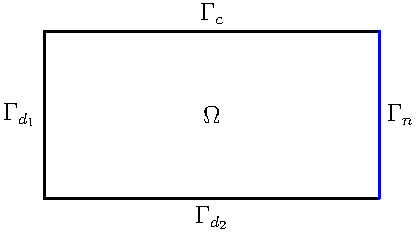
\includegraphics[width=0.6\textwidth]{burger2d_domain}
\caption{Problem domain}
\label{fig:domain}
\end{center}
\end{figure}
We consider the non-linear viscous Burgers' equation in two dimensions on the domain $\Omega = (0,1) \times (0,b)$
\begin{equation*}
w_t -\nu \Delta w + w w_{x} = f_s \qquad \mbox{in} \quad \Omega \times (0,\infty)
\end{equation*}
with boundary conditions, as shown in figure~(\ref{fig:domain})
\begin{eqnarray*}
w(0,y,t) &=& u_s \sin(\pi y/b) \qquad \mbox{ on } \Gamma_{d_1} \\
w(x,0,t) &=& 0 \qquad \mbox{ on } \Gamma_{d_2} \\
w(x,b,t) &=& u(x,t) \qquad \mbox{ on } \Gamma_c \\
\nu w_x(1,y,t) &=& g_s \sin(\pi y/b) \qquad \mbox{ on } \Gamma_n
\end{eqnarray*}
and initial condition
\begin{equation*}
w(\x,0) = w_0(\x) \quad \text{ on } \Omega
\end{equation*}
Here we denote the Dirichlet boundary as
\[
 \Gamma_d = \Gamma_{d_1} \cup \Gamma_{d_2} \cup \Gamma_c
\]

%----------------------------------------------------------------------------------------
\subsection{Observation}
We will make a Dirichlet measurement on the strip $I = [b/6,b/2]$ along the right vertical boundary, as shown in figure~(\ref{fig:obs}). Thus the observation is given by
\begin{equation*}
y_o(t) = \frac{1}{b/6} \int_{b/6}^{b/3} w(1,y,t) \ud y
\end{equation*}

\begin{figure}[h]
\begin{center}
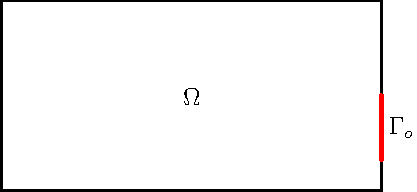
\includegraphics[width=0.6\textwidth]{burger2d_obs}
\caption{Observations}
\label{fig:obs}
\end{center}
\end{figure}

%-----------------------------------------------------------------------------------------
\subsection{Stationary Burgers' equation}
The stationary Burgers' equation is given by
\begin{equation*}
-\nu \Delta w + w w_{x} = f_s \qquad \mbox{in} \quad \Omega
\end{equation*}
with boundary conditions
\begin{eqnarray*}
w(0,y,t) &=& u_s \sin(\pi y/b) \qquad \mbox{ on } \Gamma_{d_1} \\
w(x,0,t) &=& 0 \qquad \mbox{ on } \Gamma_{d_2} \\
w(x,b,t) &=& 0 \qquad \mbox{ on } \Gamma_c \\
\nu w_x(1,y,t) &=& g_s \sin(\pi y/b) \qquad \mbox{ on } \Gamma_n
\end{eqnarray*}
An unstable stationary solution can be obtained as
\begin{equation*}
 w_s(x,y) = \tilde w_s(x) \sin{\left( \frac{\pi y}{b} \right)}
\end{equation*}
where $\tilde w_s(x)$ is the stationary solution evaluated for the one dimensional Burgers' equation
\begin{equation*}
 \tilde w_s (x) = - \frac{\nu \pi}{2} (1 + \epsilon) \tan{\left[ \frac{\pi}{4}(1+ \epsilon)x + C_0 \right]}
\end{equation*}
with
\[
\epsilon = 0.6 \qquad \Longrightarrow \qquad C_0 = \arctan(1/(1+\epsilon)) -    \frac{\pi}{4}(1 + \epsilon) = -0.69803774609235
\]
We then have
\[
u_s = \tilde{w}_s(0), \qquad g_s = \nu \dd{\tilde{w}_s}{x}(1)
\]
and $f_s$ is given by the stationary Burgers' equation.
% %-----------------------------------------------------------------------------------------
% \section{Nonlinear Burgers' equation without control}
% \begin{equation*}
% w_t -\nu w_{xx} + w w_x = f_s
% \end{equation*}
% with boundary conditions
% \begin{equation*}
% w(0,t) = u_s, \qquad w_x(1,t) = g_s
% \end{equation*}
% and initial conditions
% \begin{equation*}
% w(x,0) = w_0(x) = w_s(x) + w^\delta(x)
% \end{equation*}
% As done above, we multiply by a test function $\phi$ with $\phi(0)=0$ to obtain the weak formulation
% \[
% \int_\Omega w_t \phi \ud x + \nu \int_\Omega \dd{w}{x} \dd{\phi}{x} \ud x + \int_\Omega w \dd{w}{x} \phi \ud x = \int_\Omega f_s \phi \ud x + \nu g_s \phi(1)
% \]
% Divide domain into $N$ elements with vertices
% \[
% 0= x_0 < x < \ldots < x_N = 1, \qquad x_i = ih, \qquad h = \frac{1}{N}
% \]
% The finite element solution can be written as
% \[
% w(x,t) = \sum_{j=1}^N w_j(t) \phi_j(x) + u_s \phi_0(x)
% \]
% while the stationary solution expressed as
% \[
% w_s(x) = \sum_{j=1}^N w_s^j \phi_j(x) + u_s \phi_0(x)
% \]
% Here the $\{ \phi_j \}$ are the usual $P_1$ basis functions. The Galerkin finite element method is
% \[
% \int_\Omega w_t \phi_i \ud x + \nu \int_\Omega \dd{w}{x} \dd{\phi_i}{x} \ud x + \int_\Omega w \dd{w}{x} \phi_i \ud x = \int_\Omega f_s \phi_i \ud x + \nu g_s \phi_i(1), \qquad i=1,2,\ldots,N
% \]
% 
% \[
% f_s = \sum_{j=0}^N f_j \phi_j
% \]
% 
% \begin{eqnarray*}
% && \sum_{j=1}^N w_j'(t) \int_\Omega \phi_j \phi_i \ud x+ \nu \sum_{j=1}^N w_j(t) \int_\Omega \phi_i' \phi_j' \ud x + \sum_{j=1}^N \sum_{k=1}^N w_j(t) w_k(t) \int_\Omega \phi_i \phi_j \phi_k' \ud x \\
% && + u_s \sum_{j=1}^N w_j(t) \left[ \int_\Omega \phi_i \phi_0 \phi_j' \ud x +  \int_\Omega \phi_i \phi_j \phi_0' \ud x \right] + u_s^2 \int_\Omega \phi_i \phi_0 \phi_0' \ud x + \nu u_s \int_\Omega \phi_i' \phi_0' \ud x\\
% &=& \int_\Omega f_s \phi_i \ud x + \nu g_s \phi_i(1), \qquad i=1,2,\ldots,N
% \end{eqnarray*}
% or
% \begin{eqnarray*}
% && \sum_{j=1}^N w_j'(t) \int_\Omega \phi_j \phi_i \ud x+ \sum_{j=1}^N w_j(t) \left [ \nu \int_\Omega \phi_i' \phi_j' \ud x + u_s \int_\Omega \phi_i (\phi_0 \phi_j)' \ud x \right ] \\
% && + \sum_{j=1}^N \sum_{k=1}^N w_j(t) w_k(t) \int_\Omega \phi_j \phi_k' \phi_i \ud x \\
% &=&  - u_s^2 \int_\Omega \phi_i \phi_0 \phi_0' \ud x - \nu u_s \int_\Omega \phi_i' \phi_0' \ud x + \int_\Omega f_s \phi_i \ud x + \nu g_s \phi_i(1), \qquad i=1,2,\ldots,N
% \end{eqnarray*}
%  We use the following notations:
% \begin{itemize}
%  \item $\w = [w_1,w_2,...,w_N]^\top$
%  \item $\M \in \re^{N \times N}$ with $\M(i,j) = \int_\Omega \phi_i\phi_j \ud x$
%  \item $\A1 \in \re^{N \times N}$ with $\A1(i,j) = \int_\Omega \phi_i'\phi_j' \ud x$
%  \item $\A2 \in \re^{N \times N}$ with $\A2(i,j) = \int_\Omega \phi_i(\phi_0 \phi_j)' \ud x$
%  \item $\A = \nu \A1 + u_s \A2$
%  \item $\D1 \in \re^{N \times N \times N}$ with $\D1(i,j,k) = \int_\Omega \phi_i \phi_j' \phi_k \ud x$
%  \item $\bdd1 \in \re^{N}$ with $\bdd1(i) = \int_\Omega \phi_i \phi_0 \phi_0' \ud x$
%  \item $\bdd2 \in \re^{N}$ with $\bdd2(i) = \int_\Omega \phi_i'\phi_0' \ud x$
%  \item $\bdd3 \in \re^{N}$ with $\bdd3(i) = \int_\Omega f_s \phi_i \ud x$
%  \item $\bdd4 = [\phi_1(1), \phi_2(1), ..., \phi_N(1)]^\top \in \re^{N}$
%  \item $\bdd = -u_s^2 \bdd1 - \nu u_s \bdd2 + \bdd3 + \nu g_s \bdd4 $
% \end{itemize}
% Thus we have a system of first order system of ODEs in $\w$ which we solve using forward Euler
% \begin{eqnarray*}
%  \M \w^{n+1} = \textbf{ RHS} 
% \end{eqnarray*}
% where 
% \begin{eqnarray*}
%  \textbf{RHS}(i) = \M(i,:) \w^n + dt \left[ - A(i,:) \w^n - (W^n)^\top \D1(:,:,i) \w^n  + \bdd \right]
% \end{eqnarray*}
% 
% %-----------------------------------------------------------------------------------------
\section{Nonlinear system without control}
We set $z = w - w_s$. The equation satisfied by $z$ is
\begin{equation*}
\df{z}{t} + w_s \df{z}{x} + z \df{w_s}{x} + z \df{z}{x} = \nu \Delta z \qquad \mbox{in} \quad \Omega \times (0,\infty)
\end{equation*}
\begin{equation*}
z = 0 \quad \text{ on } \Gamma_d 
\end{equation*}
\begin{equation*}
\nu \df{z}{n} = 0 \quad \text{ on } \Gamma_n 
\end{equation*}
\begin{equation*}
z(\x,0) = w_0(\x) - w_s(\x) \quad \text{ on } \Omega
\end{equation*}
We wish to find $z \in L^2(0,T;H^1_{\Gamma_d}(\Omega))$ such that
\[
\int_\Omega z_t \phi \ud \x + \nu \int_\Omega \nabla{z} \cdotp \nabla \phi \ud \x + \int_\Omega w_s \df{z}{x} \phi \ud \x + \int_\Omega z \df{w_s}{x} \phi \ud \x + \int_\Omega z \df{z}{x} \phi \ud \x = 0
\]
for all $\phi \in H^1_{\Gamma_d}(\Omega)$

%----------------------------------------------------------------------------------------------
\subsection{FEM approximation}
Consider a division of $\Omega$ into disjoint triangles. We define the following sets of vertices
\begin{eqnarray*}
N_c &=& \mbox{vertices on $\Gamma_c$} \\
N_f &=& \mbox{interior vertices and those on $\Gamma_n$ (unknown degrees of freedom)}
\end{eqnarray*}
For each vertex $i$, define the piecewise affine functions $\phi_i(x,y)$, see figure~(\ref{fig:basis}), with the property that
\[
\phi_i(x_j, y_j) = \delta_{ij}
\]
\begin{figure}
\begin{center}
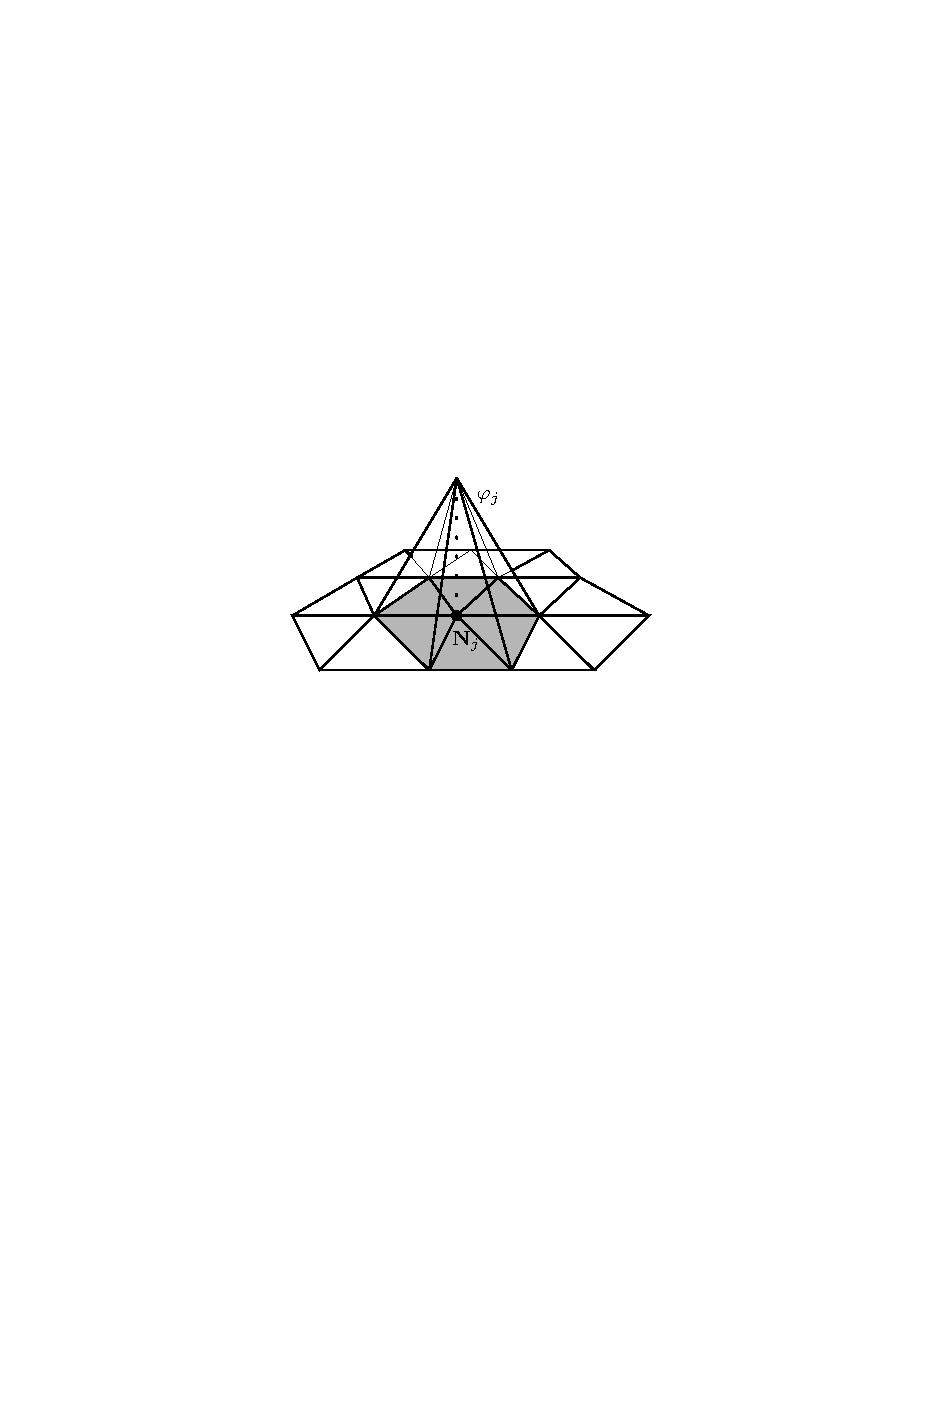
\includegraphics[width=0.5\textwidth]{tria_basis}
\caption{Piecewise affine basis functions}
\label{fig:basis}
\end{center}
\end{figure}
Thus, the finite element solution is of the form
\[
z(x,y,t) = \sum_{j \in N_f} z_j(t) \phi_j(x,y)
\]
This function satisfies the Dirichlet boundary conditions
\[
z(0,y,t) = z(x,0,t) = z(x,b,t) = 0
\]
The Galerkin method is given by
\[
\int_\Omega z_t \phi_i \ud \x + \nu \int_\Omega \nabla{z} \cdotp \nabla \phi_i \ud \x + \int_\Omega w_s \df{z}{x} \phi_i \ud \x + \int_\Omega z \df{w_s}{x} \phi_i \ud \x + \int_\Omega z \df{z}{x} \phi_i \ud \x = 0, \quad
 \forall i \in N_f
\]
i.e.,
\begin{eqnarray*}
\sum_{j \in N_f} z_j'(t) \int_\Omega \phi_i \phi_j &=& - \nu \sum_{j \in N_f} z_j(t)  \int_\Omega \nabla \phi_i \cdotp \nabla \phi_j - \sum_{j \in N_f} z_j \int_\Omega w_s \df{\phi_j}{x} \phi_i  \\
&& - \sum_{j \in N_f} z_j \int_\Omega \phi_j \df{w_s}{x} \phi_i 
 - \int_\Omega z \df{z}{x} \phi_i \\
 &=& \sum_{j \in N_f} A_{ij} z_j - \int_\Omega z \df{z}{x} \phi_i
\end{eqnarray*}
where
\[
A_{ij} = -\nu \int_\Omega \nabla \phi_i \cdotp \nabla \phi_j - \int_\Omega w_s \df{\phi_j}{x} \phi_i - \int_\Omega \phi_j \df{w_s}{x} \phi_i
\]
We can evaluate the integrals as follows.
\begin{eqnarray*}
\int_\Omega w_s \df{\phi_j}{x} \phi_i &=& \sum_{K : i,j \in K} \df{\phi_j}{x}(K) \int_K w_s \phi_i \\
&\approx& \sum_{K : i,j \in K} \df{\phi_j}{x}(K) w_s(K) \int_K \phi_i \\
&=& \sum_{K : i,j \in K} \df{\phi_j}{x}(K) w_s(K) \frac{|K|}{3}
\end{eqnarray*}

\begin{eqnarray*}
\int_\Omega \phi_j \df{w_s}{x} \phi_i &=& \sum_{K : i,j \in K} \int_K \phi_j \df{w_s}{x} \phi_i \\
&\approx& \sum_{K : i,j \in K} \df{w_s}{x}(K) \int_K \phi_j  \phi_i
\end{eqnarray*}

\begin{eqnarray*}
\int_\Omega z \df{z}{x} \phi_i &=& \sum_{K : i \in K} \int_K z \df{z}{x} \phi_i \\
&=& \sum_{K : i \in K} \df{z}{x}(K) \int_K z \phi_i \\
&=& \sum_{K : i \in K} \df{z}{x}(K) \sum_{j \in K} z_j \int_K \phi_j \phi_i 
\end{eqnarray*}
Thus we have a non-linear system of first order ODEs in $\z$
\begin{eqnarray*}
 \M \dd{\z}{t} = \A \z + N(\z) 
\end{eqnarray*}
%------------------------------------------------------------------------------------------

%\subsection{Excercises}

%\begin{enumerate}

%\item Run program {\tt nlp.m}

%\item Notice that for zero initial condition, i.e, {\tt delta = 0}, the solution will be stationary. This corresponds to the stationary solution for the original Burgers's equation.

%\item Take different initial conditions by varying {\tt delta}, and convince yourself that the zero solution is unstable. Choose values for {\tt delta} to observe the following behaviors
%   \begin{itemize}
%    \item The solution blows up
%    \item The solution converges to another steady state
%   \end{itemize}
%\end{enumerate}

%------------------------------------------------------------------------------------------

\section{Linearized Burgers' equation}

\subsection{Feedback control}
\begin{equation*}
\df{z}{t} + w_s \df{z}{x} + z \df{w_s}{x} = \nu \Delta z \qquad \mbox{in} \quad \Omega \times (0,\infty)
\end{equation*}
\begin{equation*}
z = 0 \quad \text{ on } \Gamma_d \backslash \Gamma_c, \qquad z = u \quad \text{ on } \Gamma_c
\end{equation*}
\begin{equation*}
\nu \df{z}{n} = 0 \quad \text{ on } \Gamma_n 
\end{equation*}
\begin{equation*}
z(\x,0) = w_0(\x) - w_s(\x) \quad \text{ on } \Omega
\end{equation*}
The finite element solution is of the form
\[
z(x,y,t) = \sum_{j \in N_f} z_j(t) \phi_j(x,y) + \sum_{j \in N_c} u_j(t) \phi_j(x,y), \qquad z(x_i,y_i,t) = z_i(t), \quad \forall i \in N_f
\]
This function already satisfies the Dirichlet boundary conditions
\[
z(x,0,t) = z(0,y,t) = 0, \qquad z(x,b,t) = \sum_{j \in N_c} u_j(t) \phi_j(x,b)
\]
The Galerkin method is given by
\begin{equation*}
\int_\Omega \left( \df{z}{t} + w_s \df{z}{x} + z \df{w_s}{x} \right) \phi_i = - \nu \int_\Omega \nabla z \cdotp \nabla \phi_i , \qquad i \in N_f
\end{equation*}
Ignoring the $\dd{u_j}{t}$ term gives us
\[
\sum_{j \in N_f} z_j'(t) \int_\Omega \phi_i \phi_j = \sum_{j \in N_f} A_{ij} z_j + \sum_{j \in N_c} A_{ij} u_j, \qquad i \in N_f
\]
We will take the control to be of the form
\[
u(x,t) = v(t) \sin(\pi x) \qquad \Longrightarrow \qquad u_j(t) = v(t) \sin(\pi x_j)
\]
This is a one dimensional control which is compatible with the other boundary condition on $\Gamma_{d_1}$
\[
u(0,t) = 0
\]
Then we obtain
\[
\sum_{j \in N_f} z_j'(t) \int_\Omega \phi_i \phi_j = \sum_{j \in N_f} A_{ij} z_j + \left(\sum_{j \in N_c} A_{ij} \sin(\pi x_j) \right) v, \qquad i \in N_f
\]
This can be written in matrix form as
\[
\M \dd{\z}{t} = \A \z + \B v
\]
$v(t)$ is obtained in terms of the feedback matix $\K$ 
\[
 v(t) = - \K \z
\]
The computation of $\K$ is explained in the last section.
%------------------------------------------------------------------------------------------
\subsection{Partial information with noise}
Consider the linearized model with noise in the model
\begin{equation*}
\df{z}{t} + w_s \df{z}{x} + z \df{w_s}{x} = \nu \Delta z + \eta \qquad \mbox{in} \quad \Omega \times (0,\infty)
\end{equation*}
\begin{equation*}
z = 0 \quad \text{ on } \Gamma_d \backslash \Gamma_c, \qquad z = u(t) \quad \text{ on } \Gamma_c
\end{equation*}
\begin{equation*}
\nu \df{z}{n} = 0 \quad \text{ on } \Gamma_n
\end{equation*}
\begin{equation*}
z(\x,0) = w_0(\x) - w_s(\x) \quad \text{ on } \Omega
\end{equation*}
Assume that we have access to partial information corrupted by noise
\[
y_o = Hz + \mu
\]
Using the FEM, the observation can be written as
\[
\y = \bH \z + \boldsymbol\mu
\]

%--------------------------------------------------------------------------------

\subsection{Estimation problem}
\begin{equation*}
\df{z_e}{t} + w_s \df{z_e}{x} + z_e \df{w_s}{x} = \nu \Delta z_e +  L( y - H z_e ) \qquad \mbox{in} \quad \Omega \times (0,\infty)
\end{equation*}
\begin{equation*}
z_e = 0 \quad \text{ on } \Gamma_d \backslash \Gamma_c, \qquad z_e = u(t) \quad \text{ on } \Gamma_c
\end{equation*}
\begin{equation*}
\nu \df{z_e}{n} = 0 \quad \text{ on } \Gamma_n
\end{equation*}
\begin{equation*}
z_e(\x,0) = z_0(\x) \quad \text{ on } \Omega
\end{equation*} 
In the FEM setup, we have
\[
\M \dd{\z_e}{t} = \A \z_e + \B v + \bL(\y - \bH \z_e)
\]
The computation of $\bL$ is explained in the last section.
%--------------------------------------------------------------------------------

\subsection{Coupled linear system}
The feedback is based on estimated solution $v = -\K \z_e$ which leads to the following coupled system
\begin{eqnarray*}
\M \dd{\z}{t} &=& \A \z - \B \K \z_e + \boldsymbol\eta \\
\M \dd{\z_e}{t} &=& \bL \bH \z + (\A - \B \K - \bL \bH) \z_e + \bL \boldsymbol\mu
\end{eqnarray*}
or in matrix form
\[\begin{bmatrix}
   \M & 0\\
   0 & \M \\
  \end{bmatrix}
\dd{}{t} \begin{bmatrix}
\z \\
\z_e \end{bmatrix} = \begin{bmatrix}
\A & -\B \K \\
\bL \bH & \A - \B \K - \bL \bH \end{bmatrix} \begin{bmatrix}
\z \\ \z_e \end{bmatrix} + \begin{bmatrix}
\I & 0 \\
0 & \bL \end{bmatrix} \begin{bmatrix}
\boldsymbol\eta \\ \boldsymbol\mu \end{bmatrix}
\]
The initial condition is given by
\[
\z(0) = \z_0, \qquad \z_e(0) = 0
\]
%------------------------------------------------------------------------------

\subsection{Excercises}

\begin{enumerate}
\item Compute eigenvalues of $(\A,\M)$ and check that the problem is unstable.
\item Check stabilizability and detectability using Hautus criterion.

\item Using the method given in the last section,
\begin{enumerate}

\item Compute feedback gain $\K$

\item Compute filtering gain $\bL$
\end{enumerate}

\item Solve the coupled linear system as in the 2-d heat equation case.

%\item Check stabilizabilty of $(\A,\B)$ using the Hautus criterion.

%\item Set $(\Q = 0)$ which corresponds to minimal norm control. Run the code and observe the solution and control.

%\item Set $(\Q = I)$ and run the code. How has the solution and control beaviour changed?

%\item Vary $\R$ in the range $(0.01,10)$ and observe how the feedback gain $\K$ varies.

%\item How does the solution and control change when $\nu$ is decreased?

%\item For $\Q = 0$, modify the code to solve the control and estimation problem for only the unstable components. Refer to the codes used for the 1D heat problem.
\end{enumerate}


%-----------------------------------------------------------------------------
\section{Non-linear system with control}
\begin{equation*}
\df{z}{t} + w_s \df{z}{x} + z \df{w_s}{x} + z \df{z}{x} = \nu \Delta z \qquad \mbox{in} \quad \Omega \times (0,\infty)
\end{equation*}
\begin{equation*}
z = 0 \quad \text{ on } \Gamma_d \backslash \Gamma_c, \qquad z = u(t) \quad \text{ on } \Gamma_c
\end{equation*}
\begin{equation*}
\nu \df{z}{n} = 0 \quad \text{ on } \Gamma_n 
\end{equation*}
\begin{equation*}
z(\x,0) = w_0(\x) - w_s(\x) \quad \text{ on } \Omega
\end{equation*}
The Galerkin method leads the following set of ODE
\[
\M \dd{\z}{t} = \A \z + \B v + N(\z)
\]
This model can be coupled with the linear estimator and the control is computed using the estimated solution, $v = -\K \z_e$.
%\paragraph{Excercises}

%\begin{enumerate}

%\item Run program {\tt nlp\_est.m}

%\item Vary $\R$ in the range $(0.01,10)$ and observe how the feedback gain $\K$ varies. How does the solution and control vary with $\R$.

%\item How does the solution and control change when $\nu$ is decreased?

%\end{enumerate}

%\section{List of Programs}

%\begin{enumerate}

%\item {\tt get\_system\_mat.m}: Computes FEM matrices

%\item {\tt feedback\_matrix.m}: Computes feedback matrix

%\item {\tt stationarysol.m}: Computes exact unstable stationary solution

%\item {\tt nlp.m}: Solves the non-linear model, without feedback

%\item {\tt lp\_est.m}: Solves the coupled estimation and control system for the linear problem

%\item {\tt nlp\_est.m}: Solves the coupled estimation and control system for the non-linear problem

%\item {\tt rhs\_nlp.m}: Computes the right hand side for the non-linear problem, without feedback

%\item {\tt rhs\_nlpest.m}: Computes the right hand side for coupled estimation and control system with the non-linear problem

%\end{enumerate}

%------------------------------------------------------------------------------------
\section{Control and estimation based on the unstable components}
Let $\lambda_i$ be the eigenvalues and $\V_i, \W_i$ be the eigenvectors of the pair $(\A,\M)$ and $(\A^\top,\M^\top)$ respectively.
\[
 \A \V_i = \lambda_i \M \V_i, \qquad \A^\top \W_i = \lambda_i \M \W_i, \quad \forall i = 1,...,N
\]
Assume that the eigenvectors are normalized with repsect to $\M$
\begin{equation}
 \W_i^\top \M \V_j = \delta_{i,j}, \qquad
 \W_i^\top \A \V_j = \lambda_i \delta_{i,j}
\label{eq:orthcond}
\end{equation}
Let there be $N_u$ unstable eigenvalues
\[
 Real(\lambda_{N}) < .... < Real(\lambda_{N_u +1}) < 0 < Real(\lambda_{N_u}) < ... < Real(\lambda_1)
\]
We will use the following notations 
\begin{eqnarray*}
\Lambda &=& \mbox{Diagonal matrix of eigenvalues} \\
\Lambda_u &=& \mbox{Diagonal matrix of unstable eigenvalues} \\
\V &=& \mbox{Matrix with the right eigenvector as columns} \\
\V_u &=& \mbox{Matrix with the unstable right eigenvector as columns} \\
\W &=& \mbox{Matrix with the left eigenvector as columns} \\
\W_u &=& \mbox{Matrix with the unstable left eigenvector as columns} \\
\end{eqnarray*}
\[
\V = [\V_1, \ldots, \V_N], \qquad \V_u = [\V_1, \ldots, \V_{N_u}], \qquad \W = [\W_1, \ldots, \W_N], \qquad \W_u = [\W_1, \ldots, \W_{N_u}]
\]
Consider the variable change
\[
 \z = \V \zz
\]
The system in terms of $\zz$ is written as
\[
 \M \V \dd{\zz}{t} = \A \V \zz + \B u
\]
Premultiplying by $\W^\top$ gives us
\[
 \dd{\zz}{t} = \Lambda \zz + \BB u
\]
where
\[
 \BB = \W^\top \B
\]
Projecting the system onto the unstable subspace gives
\[
 \dd{\zzu}{t} = \Lambda_u \zzu + \BBu u
\]
where
\[
\BBu = \W^\top_u \B
\]

\subsection{Control}
We find the feedback matrix for this reduced system, by solving the Bernoulli equation
\begin{equation}
 \PPu \Lambda_u + \Lambda^\top_u \PPu - \PPu \BB_u \BB_u^\top \PPu = 0
\label{eq:ricu}
\end{equation}
\[
 \Lambda_u - \BBu \BBu^\top \PPu \text{ is stable}
\]
The corresponding matrix $\bdP \in \LL(\re^{N})$ such that $(\M,\A - \B\B^\top\bdP\M)$ is stable is given by
\[
 \bdP = \W_u \PPu \V_u^\top
\]
The feedback matrix $\K$ is given by
\[
 \K = \B^\top\bdP\M
\]

\subsection{Estimation}
Define the operator $\HH$ and $\HHu$ by
\[
 \HH \zz = \bH \z, \qquad \HHu = \bH \V_u
\]
The filtering gain $\PP_e$ for the reduced projected system is obtained as the solution of the ARE
\[
 \PP_e \Lambda_u^\top + \Lambda_u \PP_e - \PP_e \HHu^\top \R_{\boldsymbol\mu}^{-1} \HHu \PP_e + \QQ_\eta = 0
\]
\[
 \Lambda_u - \PP_e \HHu^\top \R_{\boldsymbol\mu}^{-1} \HHu \text{ is stable} 
\]
where $\QQ_\eta = \W_u^\top \R_{\boldsymbol\eta} \V_u$. The corresponding $\bdP_e$ such that $(\M,\A - \M \bdP_e \bH^\top \R_{\boldsymbol\mu}^{-1} \bH)$ is stable is given by
\[
 \bdP_e = \W_u \PP_e \V_u^\top
\]
Thus the filtering gain matrix $\bdL$ is
\[
 \bdL = \M \bdP_e \bH^\top \R_{\boldsymbol\mu}^{-1}
\]
%---------------------------------------------------------------------------------------
\paragraph{Matlab tips}
To implement the above approach we need to compute only the unstable eigenvalues and eigenvectors of ($\A,\M)$ and $(\A^\top,\M^\top)$. They must also satisfy the orthonormality condition as given in equation~(\ref{eq:orthcond}). In matlab, this condition may not be automatically satisfied and you need to scale the eigenvectors appropriately.

\end{document} 

